\subsubsection{Windows 7}

Nach dem Boot wird automatisch ein neues "`RNDIS/Ethernet Gadget"' erkannt und Treiber installiert. Sollte die Installation nicht erfolgreich abgeschlossen werden k�nnen, so muss man den Treiber manuell installieren.

\begin{figure}[ht]
  \centering
  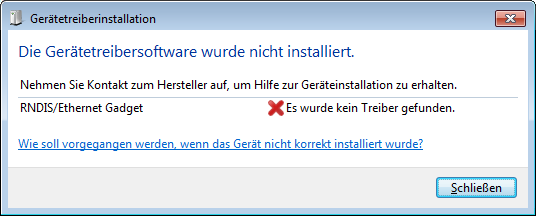
\includegraphics[scale=0.42]{images/OTG_Win7_InstallFail.png}
%  \caption{Windows Treiber konnte nicht automatisch installiert werden}
  \label{OTG_Win7_InstallFail}
\end{figure}

\begin{figure}[ht]
  \centering
  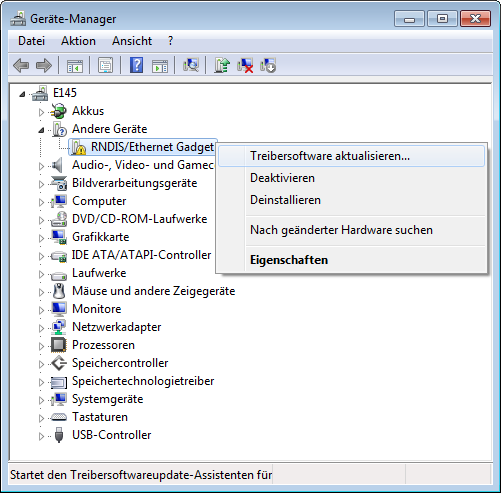
\includegraphics[scale=0.42]{images/Geraetemanager.png}
%  \caption{Windows Treiber konnte nicht automatisch installiert werden}
  \label{OTG_Win7_InstallManual}
\end{figure}

%Dazu �ffnet man den Gr�temanager, aktiviert das fehlerhafte Ger�t unter "`Andere Ger�te"' und �ffnet mit der rechten Maustaste das Kontextmen�. 
Dazu �ffnet man zuerst den Gr�temanager. Dann �ffnet man das Kontextmen� in dem man die rechten Maustatste am 
fehlerhaften Ger�t (Andere Ger�te / RNDIS/Ethernet Gadget) dr�ckt. Nun w�hlt man den Men�punkt "`Treiber Software aktualisieren..."' aus. Im folgenden Dialog w�hlt man "`Auf dem Computer nach Treibersoftware suchen"' und dann "`Aus einer Liste von Ger�tetreibern auf dem Computer ausw�hlen"'. Danach kann der Ger�tetyp gew�hlt werden in dem man "`Netzwerkadapter"' ausw�hlt. Dann w�hlt man den Hersteller "`Microsoft Corporation"' und den Netzwerkadapter "`Remote NDIS based Internet Sharing Device"'. Sollte eine Kompatibilit�tswarnung angezeigt werden, kann der Treiber trotzdem installiert werden. Zum Schluss sollte der Treiber automatisch erfolgreich installiert werden.\\ 

\begin{figure}[ht]
  \centering
  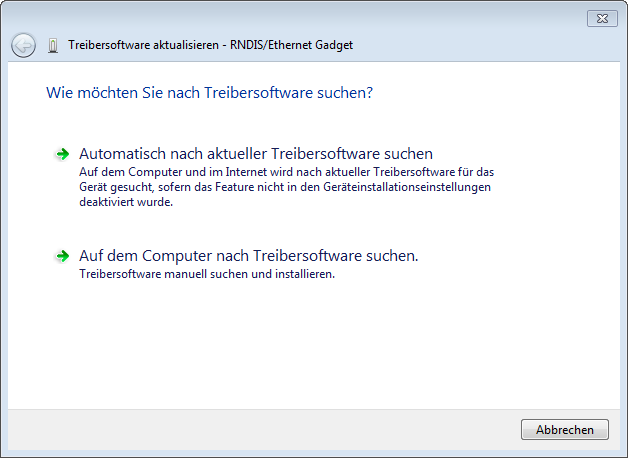
\includegraphics[scale=0.42]{images/OTG_Win7_Install_1.png}
	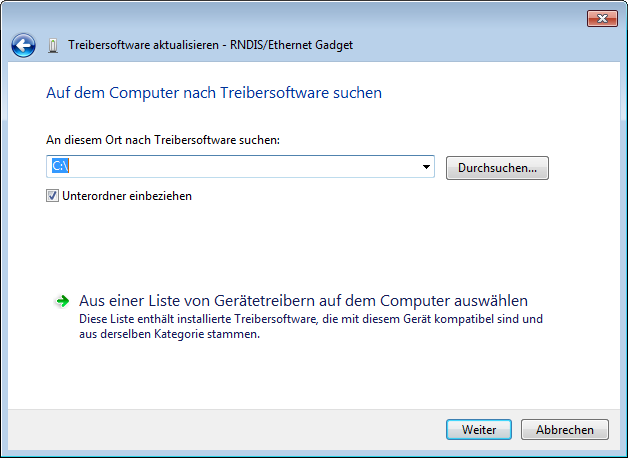
\includegraphics[scale=0.42]{images/OTG_Win7_Install_2.png}
 
%  \caption{}
  \label{OTG_Win7_Install_12}
\end{figure}

\begin{figure}[ht]
  \centering
  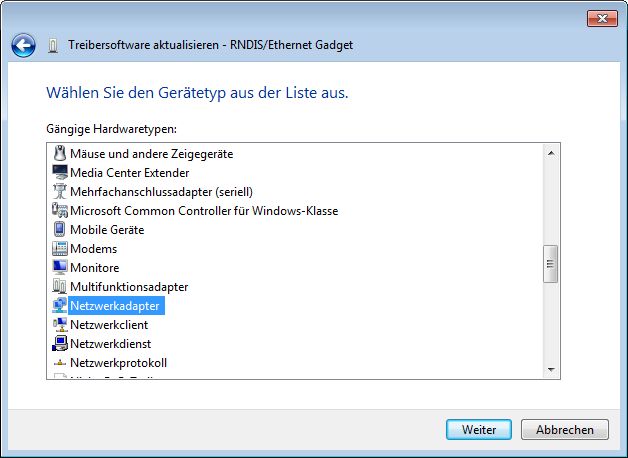
\includegraphics[scale=0.42]{images/OTG_Win7_Install_3.png}
  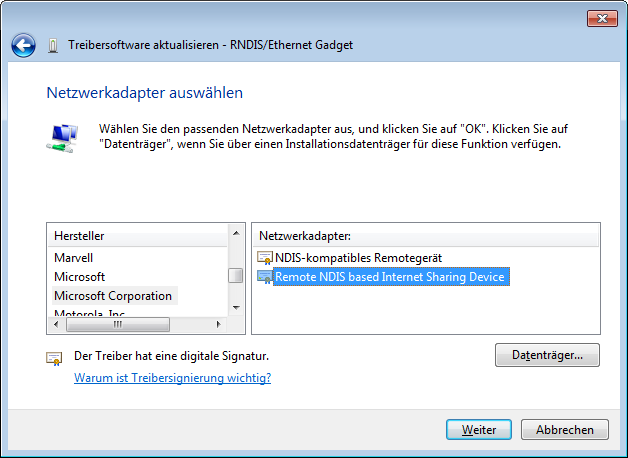
\includegraphics[scale=0.42]{images/OTG_Win7_Install_4.png}
%  \caption{}
  \label{OTG_Win7_Install_34}
\end{figure}


\begin{figure}[ht]
  \centering
  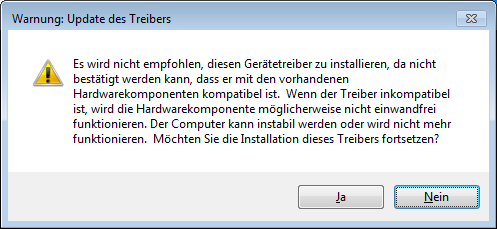
\includegraphics[scale=0.50]{images/OTG_Win7_Install_5.png}
  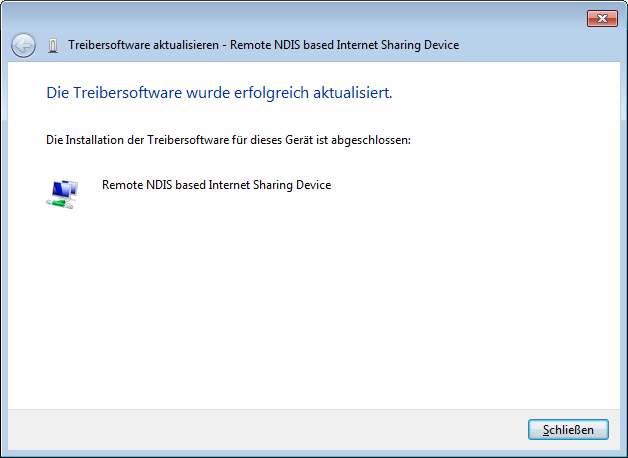
\includegraphics[scale=0.42]{images/OTG_Win7_Install_6.png}
%	\caption{}
  \label{OTG_Win7_Install_56}
\end{figure}


Damit am Ger�t Internet funktionieren kann, muss das Internet f�r das neue Netzwerk freigegeben werden. Dazu �ffnet man das Einstellungs-Fenster f�r die Netzwerkverbindungen. 

\begin{figure}[ht]
  \centering
  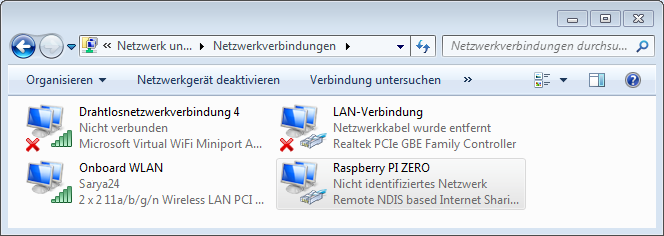
\includegraphics[scale=0.42]{images/OTG_Win7_Netzwerkverbindungen.png}
%	\caption{}
  \label{OTG_Win7_Netzwerkverbindungen}
\end{figure}

Zuerst kann man dem Netzwerkger�t "`Remote NDIS based Internet Sharing Device"' einen neuen Namen geben, z.~B. Raspberry PI ZERO. Nun muss das Netzwerk gesucht werden, das mit dem Internet verbunden ist, z.~B. Onboard WLAN. Bei den Eigenschaften zu dem Netzwerk kann der Reiter "`Freigabe"' ausgew�hlt werden. Danach kann man die Einstellung "`Anderen Benutzern im Netzwerk gestatten, diese Verbindung des Computers als Internetverbindung zu verwenden"' aktivieren und bei Heimnetzwerkverbindung kann das Netzwerk "`Raspberry PI ZERO"' ausgew�hlt werden.\\
Windows 7 legt dann fest, dass die Netzwerkadresse 192.168.137.1 sein muss. Alternativ kann die Verbindung auch zuvor schon auf diese statische IP-Adresse gesetzt werden.\\



\begin{figure}[ht]
  \centering
  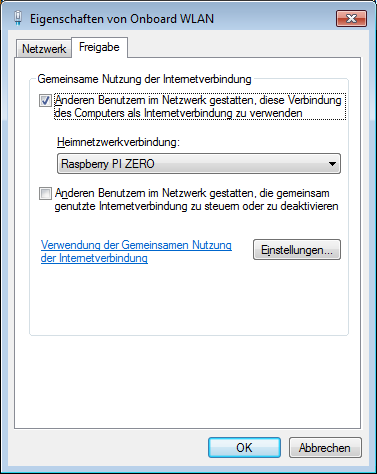
\includegraphics[scale=0.42]{images/OTG_Win7_Inet.png}
  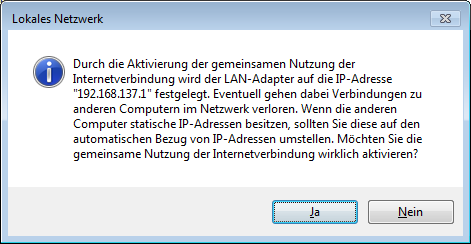
\includegraphics[scale=0.42]{images/OTG_Win7_Inet2.png}
%	\caption{}
  \label{OTG_Win7_Inet_12}
\end{figure}


Nun kann die Verbindung zur Raspberry Pi mit dem Programm Putty und der Adresse "`192.168.137.10"', �ber das SSH-Protokoll hergestellt werden.\\  
Mit dem Befehl "`ping 8.8.8.8"' kann die Internetverbindung getestet werden. Mit dem Befehl "`ping google.com"' kann dann der DNS-Server �berpr�ft werden.   
